\documentclass[10pt]{ctexbeamer}
\usepackage{ctex}
\usepackage{amsmath, amsfonts, amssymb, amsthm}
\usepackage{graphicx}
\usepackage{fontspec}
\usepackage{subfigure}
\usepackage{indentfirst}
\usepackage{graphicx}
\usepackage{multicol} %分栏
\usepackage[backend=bibtex,sorting=none]{biblatex}

\usefonttheme[onlymath]{serif}
\setbeamerfont{footnote}{size=\tiny}



\usetheme{PaloAlto}
\usecolortheme{default}

% \title{数据科学大作业汇报\\{\small _基于开源项目odoo的隐私项目扫描}}
\title[数据科学大作业]{数据科学大作业\\{\small ——基于开源项目odoo的隐私信息扫描研究}}
\author[]{殷天逸、沈霁昀、董志昂}
\date{\today}
\institute{NJU}
% \pagestyle{plain}
% \pagenumbering{arabic}



\begin{document}

    \begin{titlepage}
    \end{titlepage}

    \begin{frame}
        \frametitle{OUTLINE}
        \tableofcontents[hideallsubsections]
        
    \end{frame}

    \section{INTRODUCTION}
    \begin{frame}
        \frametitle{INTRODUCTION}
        \begin{block}{}
            在“大数据”时代,公民的隐私权保护正受到前所未有的挑战。无论是网页的cookie,还是输入的各类隐私信息,帮助软件更好的服务于我们的同时,也令人担心,我们的隐私信息是否被拿来做了其他事情。

            2021年8月20日,十三届全国人大常委会第三十次会议表决通过《中华人民共和国个人信息保护法》。其中明确对违法处理个人信息的应用程序,责令暂停或者终止提供服务。
        \end{block}
        

    \end{frame}

    \begin{frame}
        \frametitle{INTRODUCTION}
        \begin{block}{}
            本文以开源的ERP类型WEB项目Odoo(https://github.com/odoo/odoo)为研究对象,分析了其源码中与隐私信息有关的内容。Odoo主要是基于python实现的。
        \end{block}

    \end{frame}

    \begin{frame}
        \frametitle{INTRODUCTION}
        \begin{block}{}
            Odoo不仅仅是一个简单的开源ERP,Odoo更像一个框架+市场的平台,不但包含了ERP、CRM、PLM、HR等核心企业应用,还有电子商城、智能建站、社区、POS、门店管理、物流等行业应用。

            目前,各种应用的数量已经达到惊人的15850个,它的流动性和完全整合可满足甚至是最复杂公司的需求。Odoo 的灵活性在于这些应用可按照公司的发展进行添加,随着需求的变化和客户群的发展逐一添加应用。

            但也正因如此,Odoo的用户隐私信息安全就显得愈发重要,关系到诸多公司及其用户,为了研究这一问题,我们希望通过数据科学分析等方法的帮助,实现对系统隐私信息的检测。
        \end{block}
    \end{frame}

    \section{OUR WORK}
    \subsection{TASK 1}
    \begin{frame}
        \frametitle{TASK 1}
    
        \begin{block}{TASK 1}
            找到代码中的个人信息
        \end{block}
    
    \end{frame}

    \begin{frame}
        \frametitle{TASK 1}
    
        \begin{block}{实现思路}
            注意到在程序之中,个人信息往往是储存在变量之中,大部分情况下,变量名并非没有意义。在此基础之上,我们希望能够扫描了整个项目,找出源码中可能用来存储信息的变量。
        \end{block}
    \end{frame}

    \begin{frame}
        \frametitle{TASK 1}
    
        \begin{block}{实现难点}
            \begin{itemize}
                \item 对于源码中每一个的字符串,难以判断其是一个有意义的变量,还是一些没有意义的语句(如if、else...)。

                \item 此外,假如我们获取了所有的变量,识别出其中关于隐私信息的变量也是一个难点。
            \end{itemize}
        \end{block}
    \end{frame}

    \begin{frame}
        \frametitle{TASK 1}
        \begin{block}{解决方案}
            我们利用了抽象语法树(Abstract Syntax Tree,AST)来分析源码。我们借助了python的AST包,支持我们找出代码中所有的变量。
        \end{block}
    \end{frame}

    \begin{frame}
        \frametitle{TASK 1}
        \begin{block}{解决方案}
            考虑到一般来说一个项目的变量名大都较为规范,我们希望能够构建一个\textbf{隐私信息文本库},对于前文找出的所有变量,我们只需要检查其是否在文本库中,即可判断该变量是否用来存储隐私信息。
        \end{block}
    \end{frame}

    \begin{frame}
        \frametitle{TASK 1}
        \begin{block}{解决方案}
            有关文本库的构建,我们利用爬虫,抽取一些(75个左右)隐私政策作为样本,借助NLP以及一些统计方法获得这些隐私政策中的个人信息关键词,将这些关键字去重之后构成\textbf{隐私信息文本库}。

        \end{block}
    \end{frame}

    \subsection{TASK 2}
    \begin{frame}
        \frametitle{TASK 2}
        \begin{block}{TASK 2}
            找到代码中对个人信息的处理操作。
        \end{block}
    \end{frame}

    \begin{frame}
        \frametitle{TASK 2}
        \begin{block}{实现思路}
            Odoo官方在security文档(https://www.odoo.com/security)中提到,用户的数据会储存于数据库之中,因此对于个人信息的处理操作(收集、存储、使用、加工等等),都需要涉及到与数据库的交互,我们希望通过查询代码中的SQL去找到对个人信息的处理操作。
        \end{block}
    \end{frame}

    \begin{frame}
        \frametitle{TASK 2}
        \begin{block}{实现难点}
            \begin{itemize}
                \item 难以精确定位代码中的SQL。
            \end{itemize}
        \end{block}
    \end{frame}

    \begin{frame}
        \frametitle{TASK 2}
        \begin{block}{解决方案}
            我们以部分SQL语句(如INSERT)为关键词,在AST文件中进行文本匹配。我们抽取了几个样本,发现都调用了cr.execute(),其中的参数就是SQL语句。我们希望分析SQL,找到粗粒度的行为。
        \end{block}
    \end{frame}

    \subsection{TASK 3}
    \begin{frame}
        \frametitle{TASK 3}
    
        \begin{block}{TASK 3}
            对比代码行为是否符合隐私政策
        \end{block} 
    
    \end{frame}

    \begin{frame}
        \frametitle{TASK 3}
        \begin{block}{思路}
            在任务2中我们已经分析出代码对隐私信息的操作,基于此,我们认为可以通过NLP处理出隐私政策中隐私信息对应的行为,并与代码的操作进行匹配。
        \end{block}
    \end{frame}

    \begin{frame}
        \frametitle{TASK 3}
        \begin{block}{实现难点}
            \begin{itemize}
                \item 何将自然语言对隐私信息操作的描述转化为程序能理解的形式
                \item 如何将任务2中代码行为与政策中操作进行匹配,可能存在任务2中行为分析粒度过粗,无法匹配的问题。
            \end{itemize}
        \end{block}
    \end{frame}

    \begin{frame}
        \frametitle{TASK 3}
        \begin{block}{解决方案}
            如何将任务2中代码行为与政策中操作进行匹配,可能存在任务2中行为分析粒度过粗,无法匹配的问题,我们目前没有很好的解决方案。
        \end{block}
    \end{frame}

    \subsection{TASK 4}
    \begin{frame}
        \frametitle{TASK 4}
    
        \begin{block}{TASK 4}
            对获取隐私政策中的个人信息进行自动分类。
        \end{block}
    \end{frame}

    \begin{frame}
        \frametitle{TASK 4}
    
        \begin{block}{实现思路}
            在TASK 1中我们提到了\textbf{隐私信息文本库},在TASK 4中,我们希望能够借助机器学习实现对文本库中的个人信息实现精确分类。
        \end{block}
    \end{frame}

    \begin{frame}
        \frametitle{TASK 4}
        \begin{block}{实现难点}
            \begin{itemize}
                \item 敏感信息难以界定,对文本词义分类缺乏依据。
            \end{itemize}
        \end{block}
    
    \end{frame}
    
    \begin{frame}
        \frametitle{TASK 4}
        \begin{block}{解决方案}
            如果找不到训练好的分类器,我们希望能够自己训练一个。如果难度较大,我们会选择退而求其次,实现判断个人信息是否为敏感个人信息的0-1分类。
        \end{block}
    \end{frame}

    \subsection{TASK 5}
    \begin{frame}
        \frametitle{TASK 5}
        \begin{block}{TASK 5}
            判断用户数据在处理过程中是否进行过安全处理。
        \end{block} 
    \end{frame}

    \begin{frame}
        \frametitle{TASK 5}
        \begin{block}{实现思路}
            如上文所说,Odoo中的信息会储存于数据库之中,我们希望能检查其在存储到数据库的过程中是否经过加密。此外,Odoo在security文档(https://www.odoo.com/security)中还提到Odoo会对用户的密码进行加密,我们希望能找到对用户密码加密的具体操作和加密方式。
        \end{block}
    \end{frame}

    \begin{frame}
        \frametitle{TASK 5}
        \begin{block}{实现思路}
            对于加密的检测,因为常用的加密方式并不多(base64,md5,rsa等等),如果用python自带的加密需要引入相应的包,我们希望能够直接通过检查所用到的包来筛选出可能对数据进行加密操作的文件,之后再进行进一步的处理。
        \end{block}
    \end{frame}

    \section{ACHIEVEMENT DISPLAY}
    \begin{frame}
        \frametitle{ACHIEVEMENT DISPLAY}
    
        \begin{block}{部分AST}
            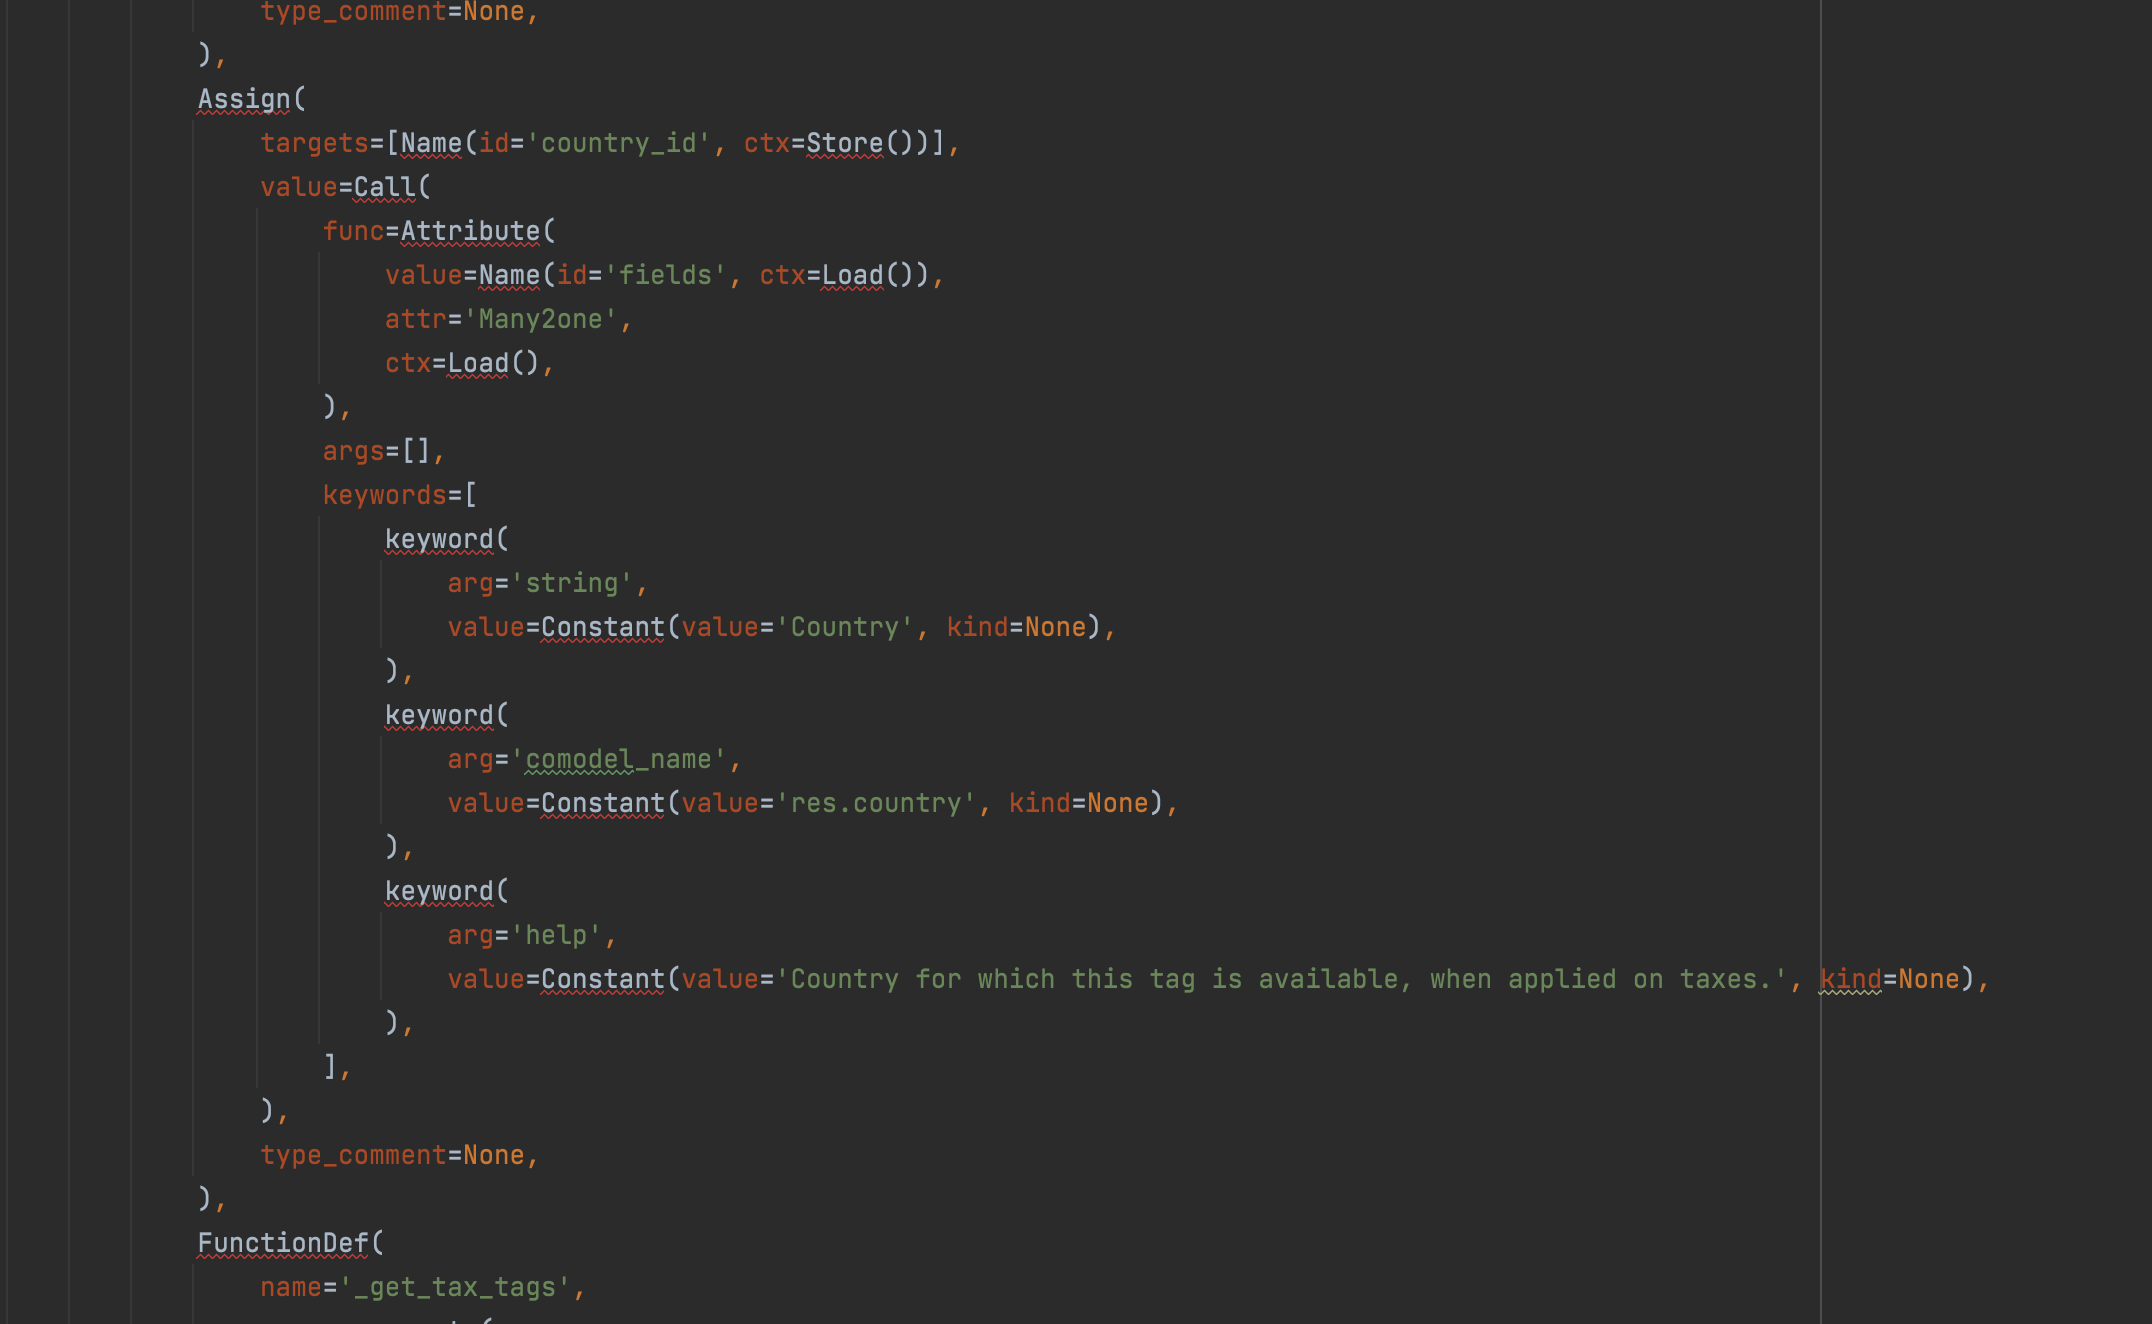
\includegraphics[scale=0.268]{AST.png}
        \end{block}
    \end{frame}

    \begin{frame}
        \frametitle{ACHIEVEMENT DISPLAY}
    
        \begin{block}{部分隐私信息文本库可视化}
            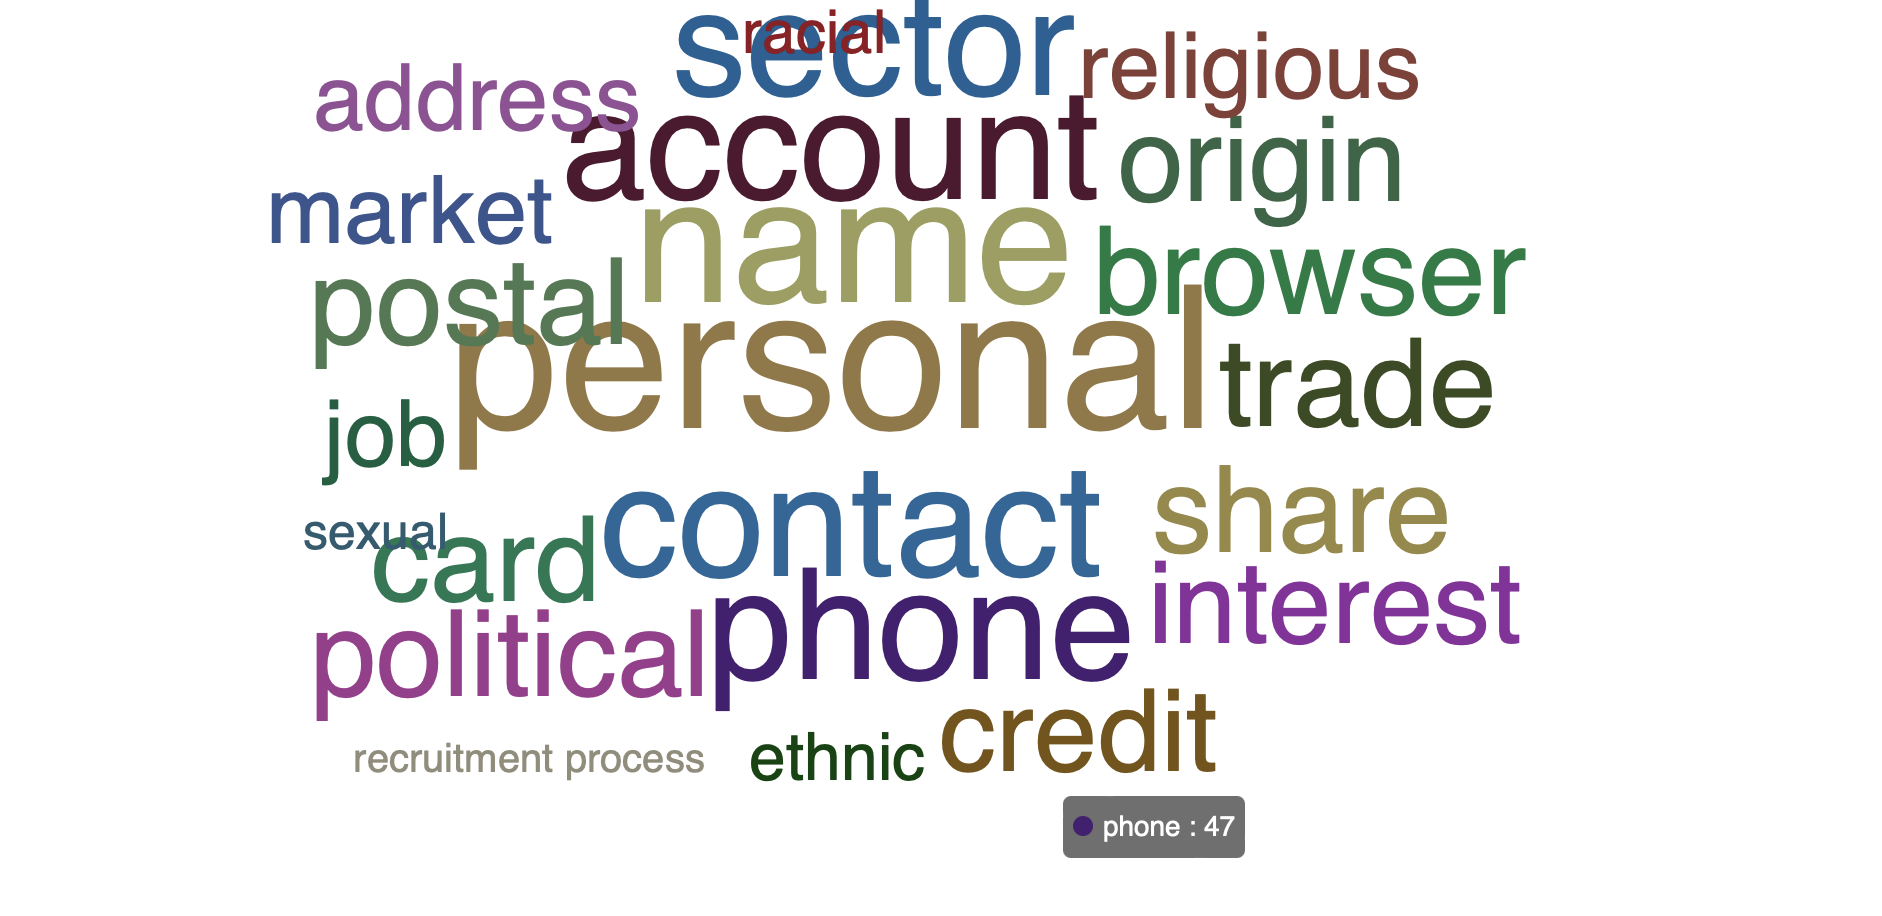
\includegraphics[scale=0.305]{dictionary.png}
        \end{block}
    \end{frame}

    \begin{frame}
        \frametitle{ACHIEVEMENT DISPLAY}
    
        \begin{block}{部分爬虫代码}
            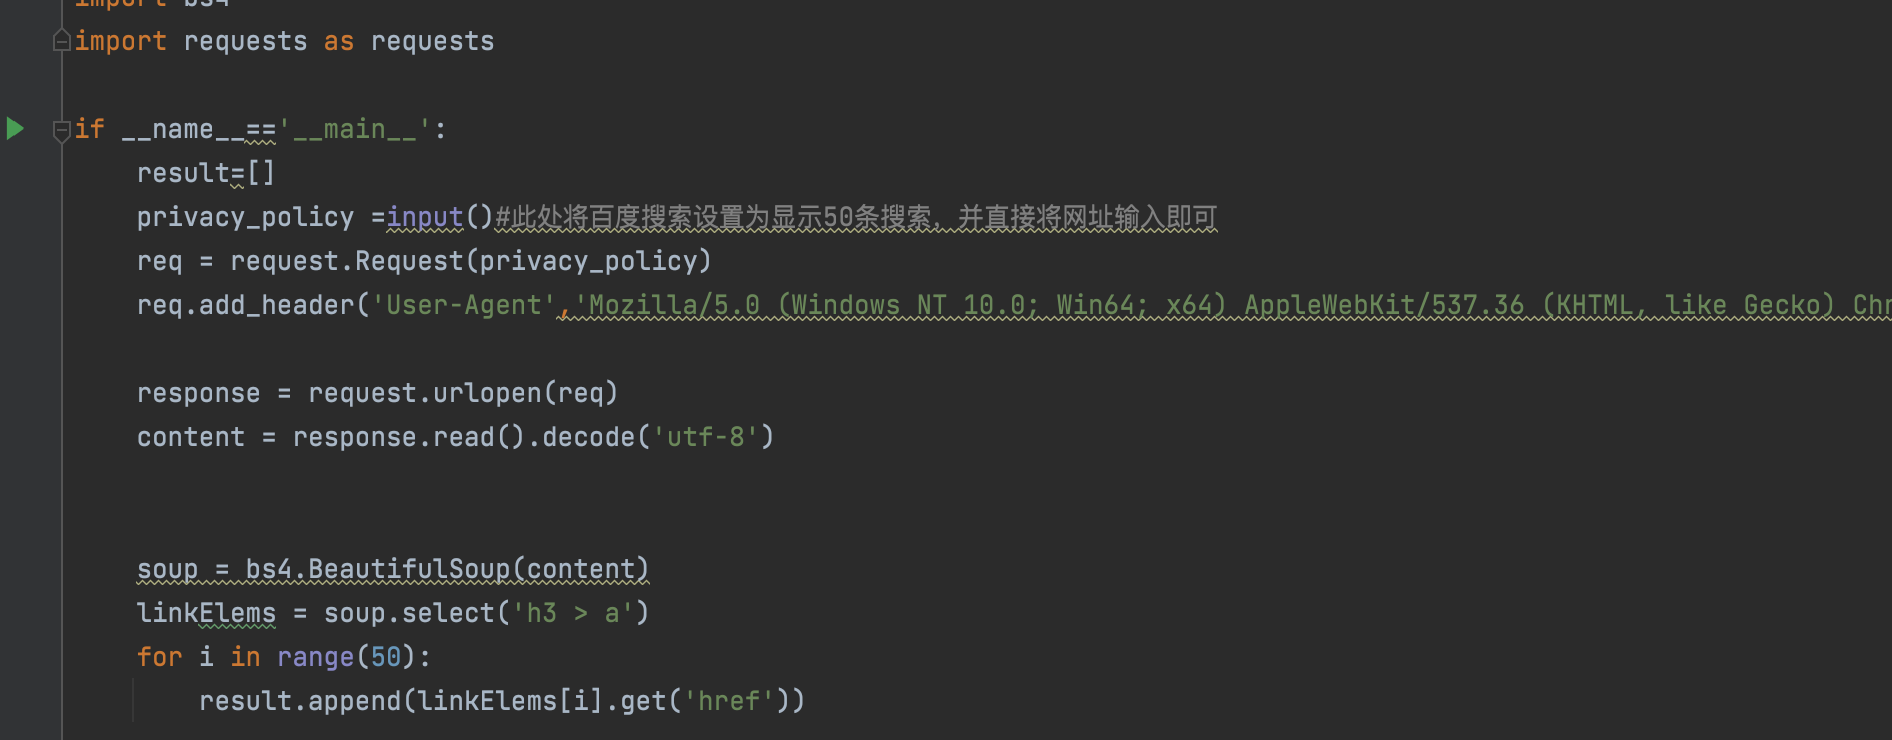
\includegraphics[scale=0.305]{crawler.png}
        \end{block}
    \end{frame}

    \begin{frame}
        \frametitle{ACHIEVEMENT DISPLAY}
    
        \begin{block}{部分NLP代码}
            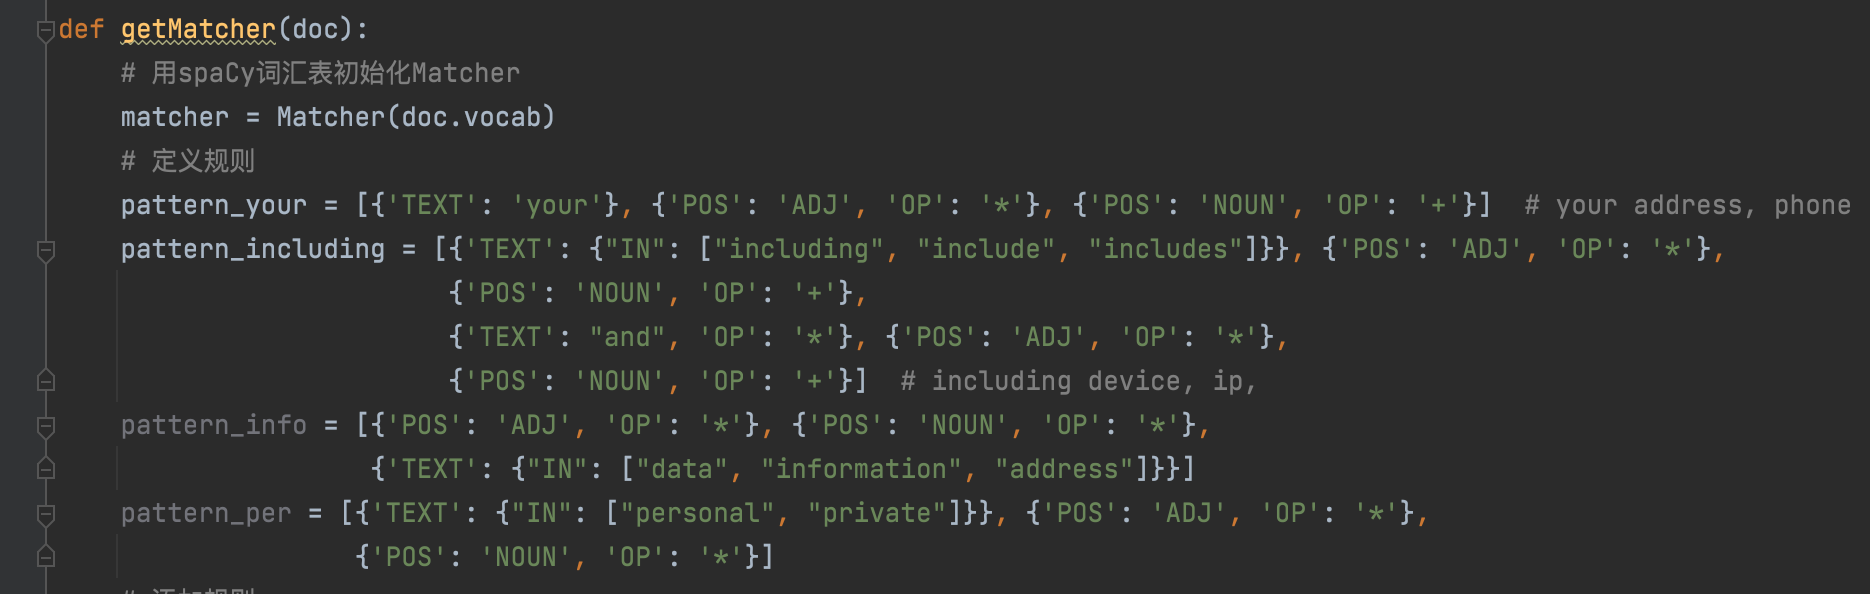
\includegraphics[scale=0.305]{nlp.png}
        \end{block}
    \end{frame}
\end{document}